% =============================================================
%  APPENDIX A — CLAP/HTS-AT ARCHITECTURE AND NOTATION
% =============================================================

\section{CLAP and HTS-AT: Architecture, Notation, and Residual Decomposition}
\label{app:architecture}

This appendix is a self-contained reference for the two components at the
core of our system. We begin by describing the CLAP dual-encoder model and
its configuration (\S\ref{app:clap_overview}). We then present the HTS-AT
audio backbone in detail, covering input preprocessing, hierarchical stage
structure, and the internal mechanics of each attention block
(\S\ref{app:htsat}). We then derive the per-head residual decomposition
that underlies our analysis (\S\ref{app:residual}). Finally, we provide
implementation details for the ResiDual spectral reweighting
(\S\ref{app:residual_impl}). All notation is introduced inline and
collected in Table~\ref{tab:notation} for reference.

% ------------------------------------------------------------------
\subsection{CLAP Overview}
\label{app:clap_overview}
% ------------------------------------------------------------------

CLAP (Contrastive Language--Audio Pretraining)~\cite{elizalde2023clap} is a
dual-encoder model that aligns audio and text representations in a shared
embedding space via contrastive learning. The audio encoder is
HTS-AT~\cite{chen2022hts} and the text encoder is
GPT-2~\cite{radford2019gpt2} (embedding dimension 768), whose weights are
frozen throughout training. Both encoders are independently projected to a
joint space of dimension $d_{\mathrm{proj}} = 1024$ via dedicated linear
projection heads; similarity is measured by temperature-scaled cosine
similarity with InfoNCE loss at temperature $\tau = 0.003$.
Zero-shot audio classification is performed by comparing an audio embedding
against the embeddings of textual class prompts.

The full configuration used in this work is reported in
Table~\ref{tab:clap_config}.

\begin{table}[h]
\centering
\caption{CLAP configuration parameters.}
\label{tab:clap_config}
\begin{tabular}{ll}
\toprule
\textbf{Parameter} & \textbf{Value} \\
\midrule
Text encoder                               & GPT-2 \\
Text encoder embedding dim                 & 768 \\
Audio encoder                              & HTS-AT \\
Audio encoder output dim ($D_3$)           & 768 \\
Joint projection dim ($d_{\mathrm{proj}}$) & 1024 \\
Contrastive temperature $\tau$             & 0.003 \\
Sampling rate                              & 44\,100\,Hz \\
Audio duration                             & 7\,s \\
Mel bands                                  & 64 \\
FFT window                                 & 1024 \\
Hop size                                   & 320 \\
$f_{\min}$ / $f_{\max}$                    & 50\,Hz / 8\,000\,Hz \\
\bottomrule
\end{tabular}
\end{table}

% ------------------------------------------------------------------
\subsection{HTS-AT Architecture}
\label{app:htsat}
% ------------------------------------------------------------------

HTS-AT~\cite{chen2022hts} is a Swin-Transformer variant adapted for audio
spectrograms. Its computation is organised into four hierarchical
\emph{stages}, each composed of several \emph{blocks}, as illustrated in
Figure~\ref{fig:htsat_architecture}. We describe the pipeline from raw audio
to the final embedding in order: input preprocessing, patch embedding, stage
structure, and the attention mechanism inside each block.

\begin{figure*}[t]
    \centering
    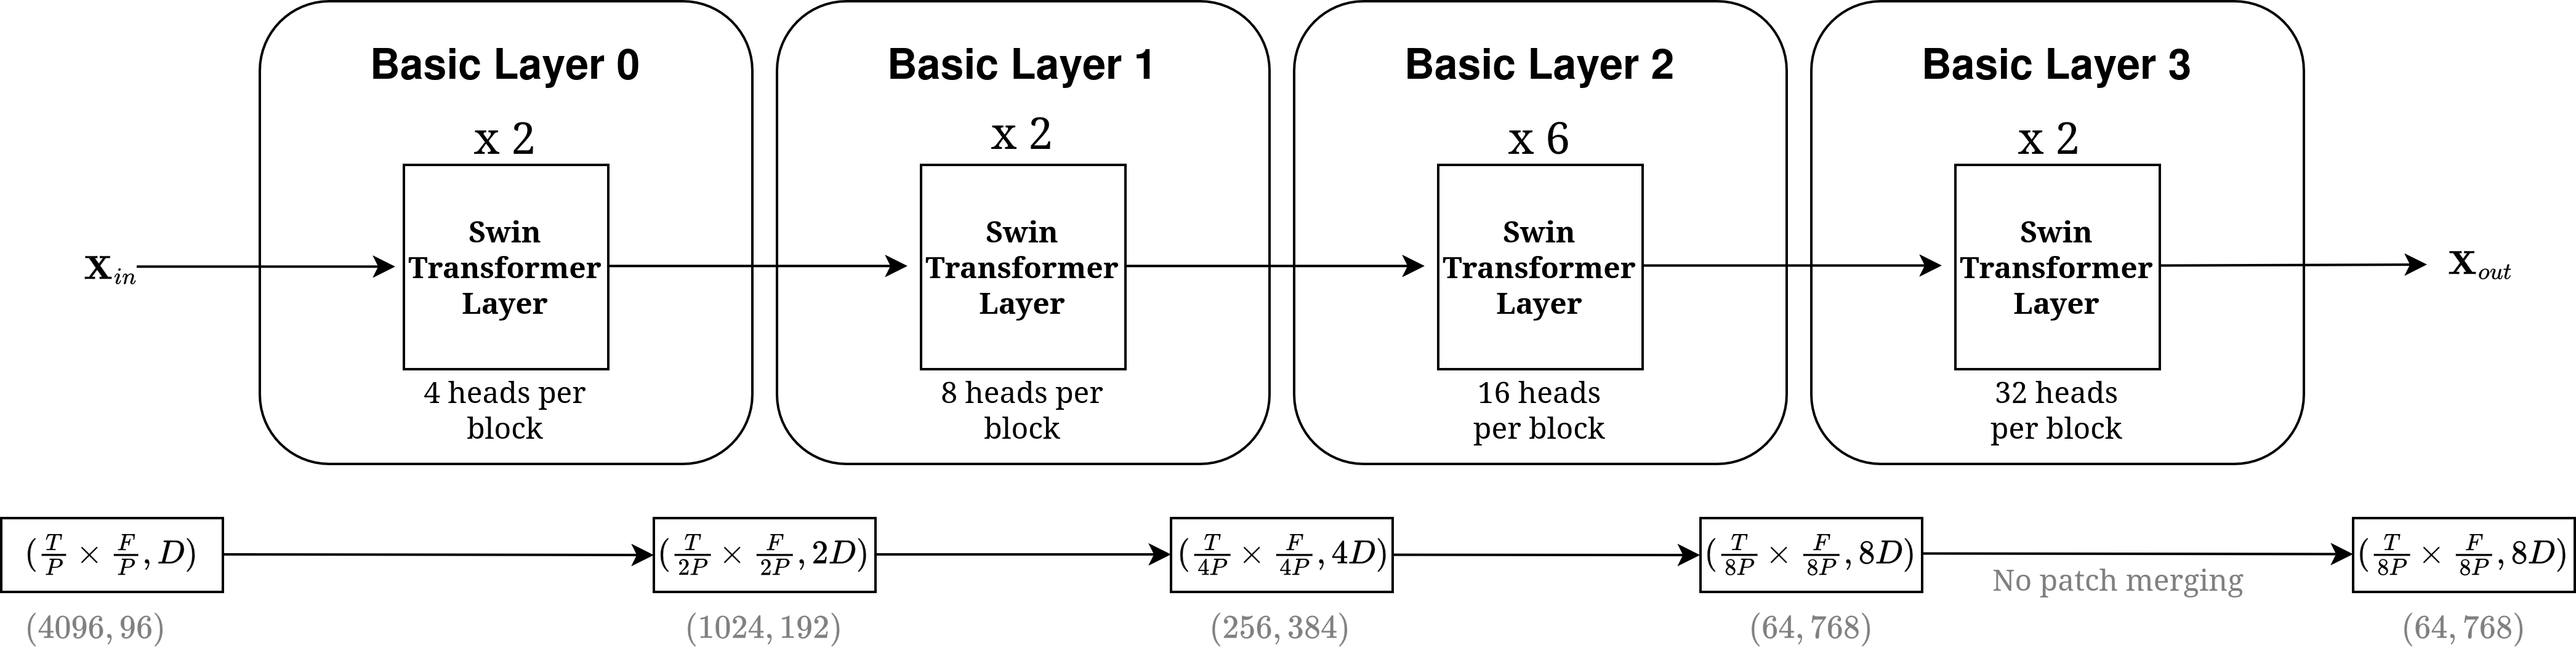
\includegraphics[width=0.95\textwidth]{images/htsat_architecture.png}
    \caption{HTS-AT hierarchical architecture. The model consists of four
        stages of increasing embedding dimension: Stage~0 (2 blocks,
        4 heads), Stage~1 (2 blocks, 8 heads), Stage~2 (6 blocks, 16 heads),
        and Stage~3 (2 blocks, 32 heads). PatchMerging is applied after
        Stages~0, 1, and~2, halving the spatial side length and doubling the
        feature dimension at each transition. Stage~3 has no PatchMerging.
        The input token sequence has spatial size $64\times64 = 4{,}096$
        tokens with embedding dimension $D_0 = 96$; after three PatchMerging
        operations the final spatial size is $8\times8 = 64$ tokens with
        $D_3 = 768$.}
    \label{fig:htsat_architecture}
\end{figure*}

\paragraph{Input preprocessing and patch embedding.}
Each audio clip is converted to a 64-band log-mel spectrogram
($f_{\min}=50$\,Hz, $f_{\max}=8{,}000$\,Hz, STFT window 1024, hop 320) and
normalised per mel-band. The resulting time--frequency matrix is rearranged
into a square image $\mathbf{x}_{\mathrm{img}} \in \mathbb{R}^{1\times256\times256}$
by folding the time axis into four contiguous segments of 256 frames stacked
vertically over the 64 mel-frequency bands ($4\times64=256$ rows, 256
columns). This image is then split into $4\times4$ non-overlapping patches
via a strided \texttt{Conv2d} layer (kernel $4\times4$, stride 4), followed
by \texttt{LayerNorm}, yielding the input token sequence
\begin{equation}
    \mathbf{Z}^{(0,0)} = \mathbf{X}_{\mathrm{in}}
    \in \mathbb{R}^{4096 \times 96},
\end{equation}
where $4096 = 64\times64$ tokens each have embedding dimension $D_0 = 96$.

\paragraph{Stage structure and PatchMerging.}
The four stages operate at progressively coarser spatial resolutions, as
summarised in Table~\ref{tab:architecture}. We index the residual stream as
$\mathbf{Z}^{(\ell,b)}$, where $\ell \in \{0,1,2,3\}$ is the stage index
and $b \in \{1,\ldots,B_\ell\}$ is the block index within that stage.

After Stages~0, 1, and~2, a \emph{PatchMerging} layer concatenates each
$2\times2$ neighbourhood of spatially adjacent tokens into a single vector of
dimension $4D_\ell$, then projects it to $2D_\ell$ via a bias-free linear
layer. This halves the spatial side length $S_\ell$ and doubles the
embedding dimension:
\begin{equation}
    \mathbb{R}^{S_\ell^2 \times D_\ell}
    \;\xrightarrow{\mathrm{PatchMerging}}\;
    \mathbb{R}^{(S_\ell/2)^2 \times 2D_\ell}.
\end{equation}
Stage~3 has no PatchMerging. The resulting spatial side lengths are
$S_\ell \in \{64, 32, 16, 8\}$ and the corresponding embedding dimensions
are $D_\ell \in \{96, 192, 384, 768\}$ (see Table~\ref{tab:architecture}).

\begin{table*}[h]
\centering
\setlength{\tabcolsep}{4pt}
\caption{HTS-AT stage-level architectural parameters. The per-head dimension
    $d_h = D_\ell / H_\ell = 24$ is constant across all stages. $S_\ell$
    is the spatial side length of the token grid at stage $\ell$;
    $N_w^\ell = S_\ell^2 / M$ is the number of attention windows, with
    $M = w^2 = 64$ tokens per window ($w=8$).}
\label{tab:architecture}
\begin{tabular}{lccccc}
\toprule
\textbf{Stage} $\ell$ & \textbf{Blocks} $B_\ell$ & \textbf{Heads} $H_\ell$ &
\textbf{Dim} $D_\ell$ & \textbf{Spatial} $S_\ell^2$ & \textbf{Windows} $N_w^\ell$ \\
\midrule
0 & 2 &  4 &  96 & $64\times64$ & 64 \\
1 & 2 &  8 & 192 & $32\times32$ & 16 \\
2 & 6 & 16 & 384 & $16\times16$ &  4 \\
3 & 2 & 32 & 768 & $8\times8$   &  1 \\
\midrule
\multicolumn{2}{l}{Total heads $H_{\mathrm{tot}}$}
    & \multicolumn{4}{l}{$2\!\cdot\!4 + 2\!\cdot\!8 + 6\!\cdot\!16 + 2\!\cdot\!32
      = 8+16+96+64 = 184$} \\
\bottomrule
\end{tabular}
\end{table*}

\paragraph{Within-stage residual structure.}
Inside each stage $\ell$, both the attention and MLP sub-layers write
additively to the residual stream. Following the pre-norm
formulation~\cite{wang2019}, the stream after block $b$ is:
\begin{equation}
    \mathbf{Z}^{(\ell,b)}
    = \mathbf{Z}^{(\ell,0)}
    + \sum_{b'=1}^{b} \mathbf{A}_{\ell,b'}
    + \sum_{b'=1}^{b} \mathbf{M}_{\ell,b'},
    \quad \in \mathbb{R}^{S_\ell^2 \times D_\ell},
    \label{eq:residual_stream}
\end{equation}
where $\mathbf{Z}^{(\ell,0)}$ is the stage input, $\mathbf{A}_{\ell,b}$ is
the W-MSA output, $\mathbf{M}_{\ell,b}$ is the MLP output, and $S_\ell$ is
the spatial side length of the token grid at stage $\ell$.

This decomposition holds strictly \emph{within} a stage, where $D_\ell$ is
constant. Across stage boundaries, PatchMerging changes both spatial
resolution and embedding dimension ($S_\ell \to S_\ell/2$,
$D_\ell \to 2D_\ell$), breaking any global additive structure across the
full network, unlike in isotropic vision transformers~\cite{gandelsman2024}.

\paragraph{Per-head output of the attention layer.}
The W-MSA output $\mathbf{A}_{\ell,b}$ is produced by concatenating the
outputs of $H_\ell$ independent attention heads and projecting through a
shared output matrix $W^O_{\ell,b}$. At block $(\ell, b)$, the raw output
of head $h$ is (see Appendix~\ref{app:htsat} for derivation):
\begin{equation}
    \mathbf{H}_{\ell,b,h}
    = \mathrm{Softmax}\!\left(
        \frac{\mathbf{Q}_h\,\mathbf{K}_h^\top}{\sqrt{d_h}}
        + \mathbf{B}_{\ell,b,h}
      \right)\mathbf{V}_h
    \;\in\; \mathbb{R}^{N_w^\ell \times M \times d_h},
    \label{eq:raw_head}
\end{equation}
where $N_w^\ell = S_\ell^2/M$ is the number of attention windows, $M=64$
tokens per window, and $\mathbf{B}_{\ell,b,h} \in \mathbb{R}^{M\times M}$
is the learned relative position bias for head $h$ at block $(\ell,b)$
(shared across windows, independent per head and per block).
All $H_\ell$ head outputs are concatenated and projected to give the W-MSA
output (see Appendix~\ref{app:residual} for the full decomposition):
\begin{equation}
    \mathbf{A}_{\ell,b}
    = \bigl[\mathbf{H}_{\ell,b,1} \|\cdots\| \mathbf{H}_{\ell,b,H_\ell}\bigr]
      \,W^O_{\ell,b} + \mathbf{b}^O_{\ell,b}
    \;\in\; \mathbb{R}^{N_w^\ell \cdot M \times D_\ell}.
    \label{eq:wmsa_out}
\end{equation}
We analyse the raw head outputs $\mathbf{H}_{\ell,b,h}$ directly,
\emph{before} the output projection $W^O_{\ell,b}$. Each
$\mathbf{H}_{\ell,b,h}$ lives in the per-head space $\mathbb{R}^{d_h}$,
which is constant across all stages and blocks. This choice avoids
entangling information across heads introduced by the shared projection, and
enables uniform cross-stage comparisons of head geometry throughout the
network. A complementary analysis of the projected contributions
$\widehat{\mathbf{H}}_{\ell,b,h}$---which characterise how each head
shapes the residual stream---is provided in Appendix~\ref{app:preprojection}.

\paragraph{Block computation: W-MSA and MLP.}
Each block $b$ at stage $\ell$ applies two sub-layers in sequence, both
preceded by LayerNorm and connected via residual additions:
\begin{align}
    \mathbf{Z}^{(\ell,b)}
        &\leftarrow \mathbf{Z}^{(\ell,b-1)} +
          \mathrm{W\text{-}MSA}_{\ell,b}\!\left(
            \mathrm{LN}\!\left(\mathbf{Z}^{(\ell,b-1)}\right)
          \right), \label{eq:residual_attn} \\[4pt]
    \mathbf{Z}^{(\ell,b)}
        &\leftarrow \mathbf{Z}^{(\ell,b)} +
          \mathrm{MLP}_{\ell,b}\!\left(
            \mathrm{LN}\!\left(\mathbf{Z}^{(\ell,b)}\right)
          \right). \label{eq:residual_mlp}
\end{align}
Even-indexed blocks use standard Window Multi-head Self-Attention (W-MSA);
odd-indexed blocks use Shifted-Window MSA (SW-MSA), which shifts the
partition by $(w/2, w/2)$ tokens to enable cross-window interactions.
At Stage~3, where $S_3 = w = 8$ so the grid coincides with a single window,
the shift degenerates to zero and all blocks use W-MSA. The MLP sub-layer
is a two-layer feed-forward network with hidden dimension $4D_\ell$ and GELU
activation.

\paragraph{WindowAttention in detail.}
The W-MSA module at block $(\ell, b)$ first partitions the $S_\ell^2$ tokens
into $N_w^\ell = S_\ell^2 / M$ non-overlapping windows of $M = 64$ tokens
each, then applies multi-head attention independently within each window.

In the SW-MSA variant, a cyclic shift is applied before window partitioning.

Queries, keys, and values are computed via a single fused projection
$W^{QKV}_{\ell,b} \in \mathbb{R}^{D_\ell \times 3D_\ell}$:
\begin{equation}
    \mathrm{LN}(\mathbf{Z}^{(\ell,b-1)})\;W^{QKV}_{\ell,b}
    \;\xrightarrow{\text{split}(D_\ell)}\;
    \mathbf{Q},\,\mathbf{K},\,\mathbf{V}
    \;\in\; \mathbb{R}^{N_w^\ell \times M \times D_\ell}.
\end{equation}
Each tensor is then reshaped to isolate the $H_\ell$ heads, yielding
per-head slices $\mathbf{Q}_h, \mathbf{K}_h, \mathbf{V}_h
\in \mathbb{R}^{N_w^\ell \times M \times d_h}$
with $d_h = D_\ell / H_\ell = 24$.

For each head $h \in \{1,\ldots,H_\ell\}$, attention is computed as:
\begin{equation}
    \mathbf{H}_{\ell,b,h}
    = \mathrm{Softmax}\!\left(
        \frac{\mathbf{Q}_h \mathbf{K}_h^\top}{\sqrt{d_h}}
        + \mathbf{B}_{\ell,b,h}
      \right)\mathbf{V}_h
    \;\in\; \mathbb{R}^{N_w^\ell \times M \times d_h},
    \label{eq:attn}
\end{equation}
where $\mathbf{B}_{\ell,b,h} \in \mathbb{R}^{M \times M}$ is the learned
relative position bias for head $h$ of block $(\ell,b)$. This bias encodes
the relative spatial offset between each pair of tokens \emph{within} a
window; it is shared across all $N_w^\ell$ windows (broadcast) and is
independent for each head. Concretely, it is read from a parameter table of
shape $((2w-1)^2, H_\ell) = (225, H_\ell)$ via a fixed index mapping, so
each head $h$ has its own column of learnable values.

All $H_\ell$ head outputs are then concatenated and passed through the
block-specific output projection $W^O_{\ell,b} \in \mathbb{R}^{D_\ell\times D_\ell}$
with bias $\mathbf{b}^O_{\ell,b} \in \mathbb{R}^{D_\ell}$, giving the
W-MSA output
\begin{equation}
    \mathbf{A}_{\ell,b}
    = \bigl[\mathbf{H}_{\ell,b,1} \|\cdots\| \mathbf{H}_{\ell,b,H_\ell}\bigr]
      \,W^O_{\ell,b} + \mathbf{b}^O_{\ell,b}
    \;\in\; \mathbb{R}^{N_w^\ell \cdot M \times D_\ell},
    \label{eq:wmsa_out}
\end{equation}
which is added to the residual stream in Eq.~\eqref{eq:residual_attn}.

% ------------------------------------------------------------------
\subsection{Per-Head Residual Decomposition}
\label{app:residual}
% ------------------------------------------------------------------

The additive residual structure of Eq.~\eqref{eq:residual_attn} allows us
to decompose the W-MSA contribution $\mathbf{A}_{\ell,b}$ exactly into
independent per-head terms. Denoting by
$W^O_{\ell,b,h} \in \mathbb{R}^{d_h \times D_\ell}$ the row slice of
$W^O_{\ell,b}$ corresponding to head $h$ (rows $[(h-1)d_h,\; hd_h)$), we
distribute the output projection over heads:
\begin{align}
    \mathbf{A}_{\ell,b}
    &= \bigl[\mathbf{H}_{\ell,b,1} \|\cdots\| \mathbf{H}_{\ell,b,H_\ell}\bigr]
       W^O_{\ell,b} + \mathbf{b}^O_{\ell,b} \notag \\
    &= \sum_{h=1}^{H_\ell}
       \Bigl(\mathbf{H}_{\ell,b,h}\,W^O_{\ell,b,h}
       + \tfrac{\mathbf{b}^O_{\ell,b}}{H_\ell}\Bigr)
    \;=\; \sum_{h=1}^{H_\ell} \widehat{\mathbf{H}}_{\ell,b,h},
    \label{eq:head_decomp}
\end{align}
where we define the \emph{per-head projected contribution}
\begin{equation}
    \widehat{\mathbf{H}}_{\ell,b,h}
    \;=\; \mathbf{H}_{\ell,b,h}\,W^O_{\ell,b,h}
          + \frac{\mathbf{b}^O_{\ell,b}}{H_\ell}
    \;\in\; \mathbb{R}^{N_w^\ell \times M \times D_\ell}.
    \label{eq:hhat}
\end{equation}
This decomposition is exact and follows from the linearity of matrix
multiplication: because $W^O_{\ell,b}$ acts on the concatenation of all
head outputs, each head $h$ effectively multiplies only its own row slice
$W^O_{\ell,b,h}$, and the output bias can be distributed equally among
heads without any approximation.

The decomposition holds within a single stage, where $D_\ell$ is constant.
Across stage boundaries, PatchMerging changes both spatial resolution and
embedding dimension, breaking any global additive structure; cross-stage
comparisons must therefore account for this.

\begin{table*}[h]
\centering
\caption{Summary of notation used throughout the paper. Symbols introduced
    by RD$^*$ are marked with $(\star)$.}
\label{tab:notation}
\begin{tabularx}{\textwidth}{llX}
\toprule
\textbf{Symbol} & \textbf{Definition} & \textbf{Values / Notes} \\
\midrule
$\ell \in \{0,1,2,3\}$
    & Stage index & \\
$b \in \{1,\ldots,B_\ell\}$
    & Block index within stage $\ell$
    & $B_\ell \in \{2,2,6,2\}$ \\
$h \in \{1,\ldots,H_\ell\}$
    & Attention head index within block $(\ell,b)$
    & $H_\ell = 4 \cdot 2^\ell \in \{4,8,16,32\}$ \\
$S_\ell$
    & Spatial side length of the token grid at stage $\ell$
    & $S_\ell \in \{64, 32, 16, 8\}$ \\
$w = 8$
    & Attention window side length & \\
$M = w^2 = 64$
    & Tokens per attention window & \\
$N_w^\ell = S_\ell^2 / M$
    & Number of attention windows at stage $\ell$
    & $N_w^\ell \in \{64, 16, 4, 1\}$ \\
$d_h = 24$
    & Per-head feature dimension (constant across stages)
    & $d_h = D_\ell / H_\ell$ \\
$D_\ell = H_\ell \cdot d_h$
    & Total embedding dimension at stage $\ell$
    & $D_\ell \in \{96, 192, 384, 768\}$ \\
$d_{\mathrm{proj}} = 1024$
    & CLAP joint embedding dimension & \\
$W^{QKV}_{\ell,b} \in \mathbb{R}^{D_\ell \times 3D_\ell}$
    & Fused QKV projection at block $(\ell,b)$ & \\
$W^O_{\ell,b} \in \mathbb{R}^{D_\ell \times D_\ell}$
    & Output projection at block $(\ell,b)$ & \\
$W^O_{\ell,b,h} \in \mathbb{R}^{d_h \times D_\ell}$
    & Row slice of $W^O_{\ell,b}$ for head $h$
    & rows $[(h-1)d_h,\; hd_h)$ \\
$\mathbf{b}^O_{\ell,b} \in \mathbb{R}^{D_\ell}$
    & Output projection bias at block $(\ell,b)$ & \\
$\mathbf{B}_{\ell,b,h} \in \mathbb{R}^{M \times M}$
    & Relative position bias for head $h$ at block $(\ell,b)$ & \\
$\mathbf{H}_{\ell,b,h} \in \mathbb{R}^{N_w^\ell \times M \times d_h}$
    & Raw head output at block $(\ell,b)$, head $h$ (pre-$W^O_{\ell,b}$) & \\
$\widehat{\mathbf{H}}_{\ell,b,h} \in \mathbb{R}^{N_w^\ell \times M \times D_\ell}$
    & Per-head projected contribution (post-$W^O_{\ell,b}$);
      see Eq.~\eqref{eq:hhat} & \\
$\mathbf{r}_{\ell,b,h} \in \mathbb{R}^{d_h}$
    & Spatially aggregated raw head output;
      see Eq.~\eqref{eq:spatial_pooling} & \\
$\widehat{\mathbf{r}}_{\ell,b,h} \in \mathbb{R}^{D_\ell}$
    & Spatially aggregated projected head output;
      see Eq.~\eqref{eq:aggregation} & \\
$\mathbf{R}_{\ell,b,h} \in \mathbb{R}^{n \times d_h}$
    & Dataset matrix of $\mathbf{r}_{\ell,b,h}$ across $n$ samples & \\
$\widehat{\mathbf{R}}_{\ell,b,h} \in \mathbb{R}^{n \times D_\ell}$
    & Dataset matrix of $\widehat{\mathbf{r}}_{\ell,b,h}$ across $n$ samples & \\
$P: \mathbb{R}^{768} \to \mathbb{R}^{1024}$
    & CLAP audio projection head (two-layer MLP with residual) & \\
$n$
    & Number of audio samples in the dataset & \\
\midrule
\multicolumn{3}{l}{\textit{Symbols introduced by RD$^*$ $(\star)$}} \\
\midrule
$\mathcal{L} \subseteq \{0,1,2,3\}$ $(\star)$
    & Target stage indices for reweighting
    & Default $\{1, 2, 3\}$ \\
$\rho_{\mathrm{var}} \in (0,1)$ $(\star)$
    & Variance threshold for per-head subspace estimation
      (Eq.~\eqref{eq:k_threshold})
    & Default $0.95$ \\
$k_{\ell,b,h} \in \{1,\ldots,d_h\}$ $(\star)$
    & Number of task-relevant PCA components for head $h$ at block
      $(\ell,b)$, determined by $\rho_{\mathrm{var}}$
      (Eq.~\eqref{eq:k_threshold}) & \\
$\boldsymbol{\lambda}_{\ell,b,h} \in \mathbb{R}^{d_h}$ $(\star)$
    & Learnable per-component weight vector for head $h$ at block $(\ell,b)$;
      initialised via Eq.~\eqref{eq:lambda_init},
      optimised via Eq.~\eqref{eq:optim_obj}
    & \texttt{nn.Parameter} \\
$\mathbf{C}_{\ell,b,h} \in \mathbb{R}^{d_h \times d_h}$
    & Empirical covariance matrix of $\widetilde{\mathbf{R}}_{\ell,b,h}$
    & See Eq.~\eqref{eq:pca_decomp} \\
$\boldsymbol{\Phi}_{\ell,b,h} \in \mathbb{R}^{d_h \times d_h}$
    & Orthogonal matrix of eigenvectors of $\mathbf{C}_{\ell,b,h}$
    & Columns ordered by
      $\lambda^{\mathrm{ev}}_1 \ge \cdots \ge \lambda^{\mathrm{ev}}_{d_h}$ \\
$\lambda^{\mathrm{ev}}_j$
    & $j$-th eigenvalue of $\mathbf{C}_{\ell,b,h}$,
      $\lambda^{\mathrm{ev}}_1 \ge \cdots \ge \lambda^{\mathrm{ev}}_{d_h} \ge 0$
    & Fixed after fitting pass; not trainable \\
$\boldsymbol{\mu}_{\ell,b,h} \in \mathbb{R}^{d_h}$
    & Empirical mean of $\widetilde{\mathbf{R}}_{\ell,b,h}$
    & Fixed buffer; not trainable \\
$\widetilde{\mathbf{R}}_{\ell,b,h} \in \mathbb{R}^{N_{\mathrm{fit}} \times d_h}$
    & Fitting matrix for head $h$ of block $(\ell,b)$
    & See Eq.~\eqref{eq:fitting_matrix} \\
$N_{\mathrm{fit}}$
    & Total rows of the fitting matrix;
      $N_{\mathrm{fit}} = \sum_{\mathrm{batches}} B \cdot N_w^\ell \cdot M$ & \\
$N_{\max}$
    & Maximum number of audio clips used in fitting pass
    & Default $10\,000$ \\
$\widetilde{\mathbf{H}}_{\ell,b,h} \in \mathbb{R}^{B' \times N \times d_h}$
    & Centred head output $(\mathbf{H}_{\ell,b,h} - \boldsymbol{\mu}_{\ell,b,h})$ & \\
$\mathbf{Z}_{\ell,b,h} \in \mathbb{R}^{B' \times N \times d_h}$
    & Projection of $\widetilde{\mathbf{H}}_{\ell,b,h}$ onto the full PCA basis
    & \\
$\widehat{\mathbf{Z}}_{\ell,b,h} \in \mathbb{R}^{B' \times N \times d_h}$
    & Rescaled PCA projection
      ($\mathbf{Z}_{\ell,b,h} \odot \boldsymbol{\lambda}_{\ell,b,h}^\top$)
    & See Eq.~\eqref{eq:rd_reweight} \\
$\mathbf{H}^*_{\ell,b,h} \in \mathbb{R}^{B' \times N \times d_h}$
    & Reweighted head output; replaces $\mathbf{H}_{\ell,b,h}$
      in Eq.~\eqref{eq:wmsa_out}
    & See Eq.~\eqref{eq:reweighted_head} \\
$\hat{\mathbf{a}}(x) \in \mathbb{R}^{d_{\mathrm{proj}}}$
    & $\ell_2$-normalised audio embedding used in the optimisation objective
    & See Eq.~\eqref{eq:optim_obj} \\
$\mathbf{t}_c \in \mathbb{R}^{d_{\mathrm{proj}}}$
    & $\ell_2$-normalised text embedding of class $c$
    & Pre-computed; fixed during optimisation \\
$\mathcal{J}(\boldsymbol{\lambda})$
    & Cross-entropy zero-shot loss (Eq.~\eqref{eq:optim_obj})
    & Minimised over validation set \\
$\eta$
    & Learning rate for Schedule-Free Adam
    & Default $10^{-2}$ \\
$p$
    & Early-stopping patience (epochs without improvement)
    & Default $5$ \\
$T_{\max}$
    & Maximum number of optimisation epochs
    & Default $30$ \\
\bottomrule
\end{tabularx}
\end{table*}